\section{The Nudged Elastic Band Method}
\label{sec:neb}

Finding Steepest Decent Paths (SDPs) on a multidimensional function, $V(\vR)$, from a given point is simple by following the negative gradient (force) with a small step size.
On the other hand, finding specific SDPs that end at minima is not.
The Nudged Elastic Band (NEB) algorithm is concerned with aligning a path with certain SDP paths, genreally the MEP (see~\cite{neb-polemic-henkelman1} for an exeption), leading to two minima from a common \sap{1}.

\begin{figure}[h]
\begin{center}
    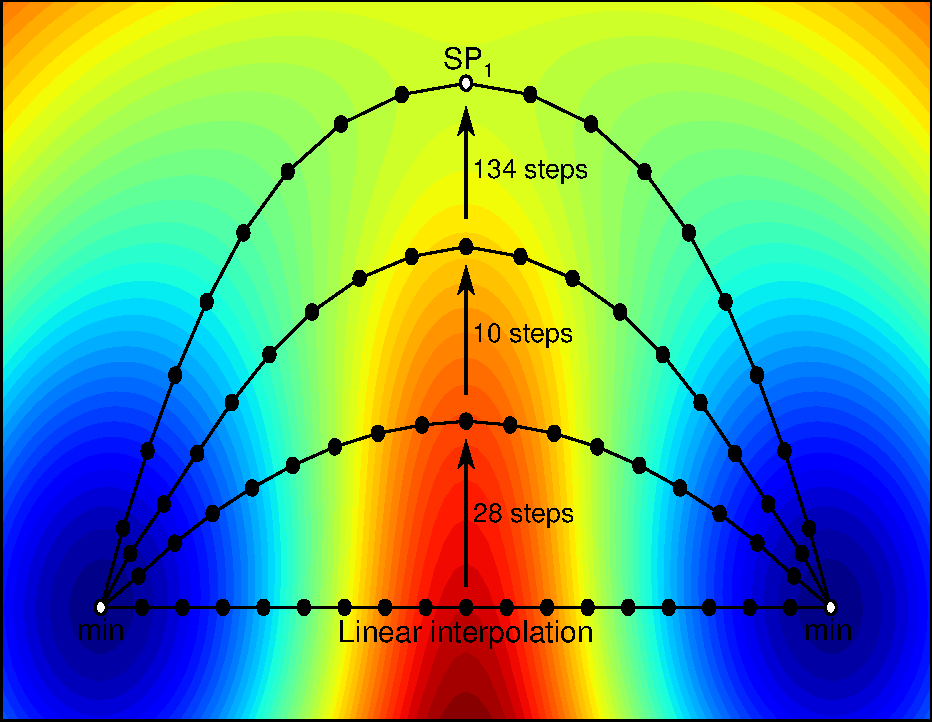
\includegraphics[width=0.6\linewidth]{neb-pes-paths}
\parbox{0.85\linewidth}{\caption{Snapshots from a NEB optimisation of a MEP.
Each series of connected circles (the images) represents the path at a specific iteration step.
The white circles are stationary points, two minima and a \sap{1}.
Red and blue areas represent high and low values of the function in question, respectively.}
\label{fig:neb-pes-paths}}
\end{center}
\end{figure}

\subsubsection{The Force Modification Scheme}
An initial guess of the path is commonly a, discretisised, linear interpolation bewteen the minima but any guess is suitable as long as the force can be calculated.
Each of the discretisation points is, traditionally, referred to as an image and is simply a replica of the system in question but with different coordinates from the other images.
Each image, $i$, feels two separate forces.
First there is the negative gradient of the function, $\vF_i \equiv -\nabla V(\vR_i)$, but only the component perpendicular to the path is retained,
\beq{neb-real-force}
\vF_i^\perp = \vF_i - (\vF_i \cdot \uvt_i) \uvt_i,
\eeq
where $\uvt$ is the tangent to the path (see below).
This reduced force is responsible for minimising the path in the perpendicular direction.
Second, there is a virtual force acting purely along the tangent, which is tasked with equally spacing the images along the path.
There are multiple ways to implement this force, the original implementation of NEB~\cite{neb-original-1998} modelled a spring between each set of neighboring images with a tunable spring constant, $k$.
A more recent, and succesful, version of the "spring force", depends on the norms to the neighboring images instead of the full vectors~\cite{neb-tangent-2000},
\beq{neb-spring-force}
\vF_i^\text{S} = k(\left| \vR_{i+1} - \vR_i \right| - \left| \vR_i - \vR_{i-1}\right|),
\eeq
where $k$, is still present as a stiffness parameter.
By varying the stiffness parameter for each image, it is possible to increase the density of images in interesting areas, such as near the \sap{1}.~\cite{neb-ci-2000}

Combining the forces from equations \ref{eq:neb-real-force} and \ref{eq:neb-spring-force} into an effective force, as seen in \fref{fig:neb-force-overview},
\beq{neb-effective-force}
\vF_i^\text{eff} = \vF_i^\perp + \vF_i^\text{S},
\eeq
will iteratively bring the path to a discretisised version of the MEP, with even, or controlled, spacing, as can be seen in \fref{fig:neb-pes-paths}.

\begin{figure}[h]
\begin{center}
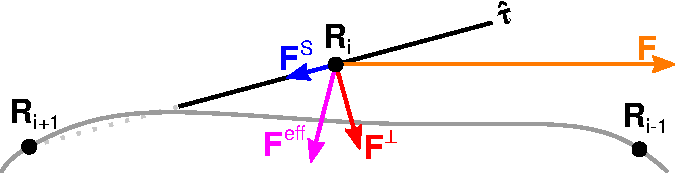
\includegraphics[width=0.6\linewidth]{neb-force-overview}
\parbox{0.85\linewidth}{\caption{A schematic overview of the force components acting within the NEB method.
$\vR_{i-1}$, $\vR_i$ and $\vR_{i+1}$ are the positions of each image.
The label $i$ is ommited from the force symbols as all of them originate at image number $i$.
$\vF$ (orange) is the gradient force,
$\vF^\perp$ (red) is the force perpendicular to the tangent (\fref{eq:neb-real-force}),
$\vF^\text{S}$ (blue) is the spring force (\fref{eq:neb-spring-force}) and
$\vF^\text{eff}$ (purple) is the effective force (\fref{eq:neb-effective-force}).
The tangent, $\uvt$, is the unit vector pointing towards the neighboring, higher function value, image, $i+1$ (\fref{eq:neb-tangent-plus}).
}
\label{fig:neb-force-overview}
}
\end{center}
\end{figure}

\subsubsection{Tangent}
Since the path must be discretisised, the tangent can not be trivially defined.
Multiple possibilities for its definition are available but one that considers only the displacement to the neighboring, higher function value, image has been succesful in minimising kinks in the paths.~\cite{neb-tangent-2000}

Each image, $i$, will, function value wise, fit into one of four cases:
\ben{neb-tangent-cases}
\item $V(\vR_{i-1}) < V(\vR_i) < V(\vR_{e+1})$
\item $V(\vR_{i-1}) > V(\vR_i) > V(\vR_{e+1})$
\item $V(\vR_{i-1}) > V(\vR_i) < V(\vR_{e+1})$
\item $V(\vR_{i-1}) < V(\vR_i) > V(\vR_{e+1})$
\een
Before discussing each case it is helpful to define vectors to the neighboring images:
\beq{tangent-plus}
\vt_i^+ = \vR_{i+1} - \vR_i \quad \text{and} \quad \vt_i^- = \vR_i - \vR_{i-1}.
\eeq
The first two cases yield simple definitions of the tangent,
\beq{neb-tangent-plus}
\uvt_i = \frac{\vt_i^+}{\left| \vt_i^+ \right|} \quad \text{if} \quad V(\vR_{i-1}) < V(\vR_i) < V(\vR_{e+1})
\eeq
and
\beq{neb-tangent-minus}
\uvt_i = \frac{\vt_i^-}{\left| \vt_i^- \right|} \quad \text{if} \quad V(\vR_{i-1}) > V(\vR_i) > V(\vR_{e+1}).
\eeq
The other two cases occur when the image is either a local maximum or a local minimum, with regards to its neighboring images.
In these latter cases a weighted average
--- controlled by the difference in the function's value, $\Delta{}E = \left[ \left| V(\vR_{i+1}) - V(\vR_i) \right|, \left| V(\vR_{i-1}) - V(\vR_i) \right| \right]$ ---
of the neighboring tangents is used, in order to avoid any artifacts due to discontinuity,
\beq{neb-tangent-minmax}
\uvt_i = \frac{\vt_i^+ \upsilon_i^\pm + \vt_i^- \upsilon_i^\mp}{\left| \vt_i^+ \upsilon_i^\pm + \vt_i^- \upsilon_i^\mp \right|} \quad \text{if} \quad E(\vR_{i\pm1}) > V(\vR_{i\mp1}),
\eeq
where $\upsilon_i^+ = \text{max}(\Delta{}E)$ and $\upsilon_i^- = \text{min}(\Delta{}E)$ are the weights.

\subsubsection{Finding the Exact Saddle Point}
The force modifications described above do not guarantee that an image will be exactly at the \sap{1} in question once converged.
By decoupling the top function value image from the spring force, it becomes independant and guiding it to the \sap{1} can be done in a manner similar to \fref{eq:dimer-transform} with the tangent estimate functioning as the minimum mode estimate,
\beq{neb-ci-transform}
\vF_{i_\text{max}}^\text{eff} = \vF_i - (\vF_i \cdot \uvt_i)\uvt_i,
\eeq
where $i_\text{max}$ refers to the image with the highest function value.~\cite{neb-ci-2000}

\subsubsection{Usage in Atomic Simulations}

\placeholder

